\documentclass[11pt,a4paper]{article}
\usepackage[margin=1in]{geometry}
\usepackage{amsmath,amssymb}
\usepackage{graphicx}
\usepackage{booktabs}
\usepackage{hyperref}
\usepackage{xcolor}
\usepackage{tikz}
\usetikzlibrary{arrows.meta,positioning,shapes.geometric,fit,backgrounds,calc}
\usepackage{listings}
\usepackage{enumitem}
\usepackage{float}
\usepackage{caption}

\lstset{
  basicstyle=\ttfamily\small,
  backgroundcolor=\color{gray!10},
  frame=single,
  breaklines=true,
  columns=fullflexible,
}

\hypersetup{
  colorlinks=true,
  linkcolor=blue!60!black,
  citecolor=blue!60!black,
  urlcolor=blue!60!black,
}

\title{Integrating Temporal Memory into GraphCast:\\Architecture Overview and Alternative Approaches}
\author{Lianghong Mo}
\date{April 2026}

\begin{document}
\maketitle

\begin{abstract}
GraphCast is a state-of-the-art graph neural network for medium-range weather forecasting. It operates autoregressively but lacks explicit temporal memory across prediction steps. This document provides a self-contained overview of the GraphCast architecture, explains how we integrate a Mamba selective state space model to provide cross-rollout memory, presents our experimental findings (the approach does not yet outperform the baseline), and discusses alternative temporal memory mechanisms that may be more effective.
\end{abstract}

\tableofcontents
\newpage

%=============================================================================
\section{GraphCast: Architecture}
%=============================================================================

\subsection{The Weather Prediction Problem}

Numerical weather prediction (NWP) aims to forecast the future atmospheric state given the current and recent observations. The atmosphere is described by a set of physical variables---temperature, wind components, humidity, pressure, geopotential---at discrete grid points across the globe and at multiple pressure levels (altitudes).

Traditional NWP solves partial differential equations (Navier-Stokes, thermodynamics) on a computational grid. GraphCast~\cite{lam2023graphcast} replaces this with a learned mapping: given the atmospheric state at two consecutive time steps ($t{-}\Delta t$ and $t$, where $\Delta t = 6\text{h}$), predict the state at $t{+}\Delta t$.

\subsection{The Encode-Process-Decode Framework}

GraphCast follows an encode-process-decode structure, using an icosahedral mesh as a latent spatial representation:

\begin{figure}[H]
\centering
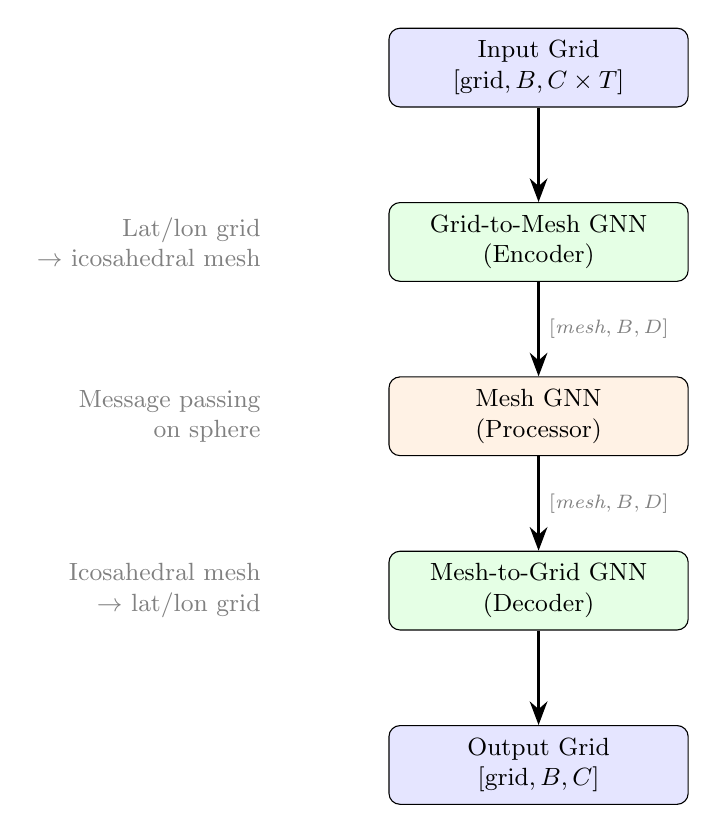
\begin{tikzpicture}[
  box/.style={draw, rounded corners, minimum width=3.8cm, minimum height=1.0cm, align=center, font=\small},
  arrow/.style={-{Stealth[length=3mm]}, thick},
  label/.style={font=\scriptsize\itshape, text=gray},
]

% Nodes
\node[box, fill=blue!10] (input) {Input Grid\\$[\text{grid}, B, C \times T]$};
\node[box, fill=green!10, below=1.2cm of input] (g2m) {Grid-to-Mesh GNN\\(Encoder)};
\node[box, fill=orange!10, below=1.2cm of g2m] (mesh) {Mesh GNN\\(Processor)};
\node[box, fill=green!10, below=1.2cm of mesh] (m2g) {Mesh-to-Grid GNN\\(Decoder)};
\node[box, fill=blue!10, below=1.2cm of m2g] (output) {Output Grid\\$[\text{grid}, B, C]$};

% Arrows
\draw[arrow] (input) -- (g2m);
\draw[arrow] (g2m) -- (mesh) node[midway, right, label] {$[\text{mesh}, B, D]$};
\draw[arrow] (mesh) -- (m2g) node[midway, right, label] {$[\text{mesh}, B, D]$};
\draw[arrow] (m2g) -- (output);

% Side labels
\node[left=1.5cm of g2m, font=\small, text=gray, align=right] {Lat/lon grid\\$\to$ icosahedral mesh};
\node[left=1.5cm of mesh, font=\small, text=gray, align=right] {Message passing\\on sphere};
\node[left=1.5cm of m2g, font=\small, text=gray, align=right] {Icosahedral mesh\\$\to$ lat/lon grid};

\end{tikzpicture}
\caption{GraphCast's encode-process-decode pipeline for a single prediction step.}
\label{fig:graphcast}
\end{figure}

\subsubsection{Step 1: Input Feature Construction}

The input consists of $T$ consecutive atmospheric snapshots (typically $T{=}2$). All time steps are \textbf{concatenated along the channel dimension}:
\[
\mathbf{f}_i = [\mathbf{x}_{t-\Delta t}^{(i)} \;;\; \mathbf{x}_{t}^{(i)}] \in \mathbb{R}^{2C}
\]
where $i$ indexes the $N_\text{grid}$ latitude-longitude grid nodes. This simple concatenation allows a downstream MLP to learn temporal features such as:
\begin{itemize}[nosep]
  \item Velocity: $\mathbf{x}_t - \mathbf{x}_{t-\Delta t}$
  \item Acceleration (with $T{=}4$): $(\mathbf{x}_t - \mathbf{x}_{t-\Delta t}) - (\mathbf{x}_{t-\Delta t} - \mathbf{x}_{t-2\Delta t})$
  \item Any nonlinear combination of the concatenated frames
\end{itemize}

\subsubsection{Step 2: Grid-to-Mesh Encoder}

A graph neural network maps features from the regular lat/lon grid to an \textbf{icosahedral mesh}---a hierarchical triangulation of the sphere. The mesh provides:
\begin{itemize}[nosep]
  \item \textbf{Uniform spatial sampling}: Unlike lat/lon grids (which cluster at the poles), icosahedral meshes have approximately uniform node spacing.
  \item \textbf{Efficient global communication}: At coarse mesh levels, adjacent nodes span large geographic distances, enabling information to propagate globally in few message-passing steps.
\end{itemize}

The encoder performs one message-passing step on a bipartite graph connecting grid nodes to their nearest mesh nodes:
\[
\mathbf{m}_j = \text{GNN}_\text{encode}\left(\{\mathbf{f}_i\}_{i \in \mathcal{N}(j)}\right) \in \mathbb{R}^D
\]
where $j$ indexes mesh nodes and $\mathcal{N}(j)$ are grid nodes within a query radius.

\subsubsection{Step 3: Mesh Processor}

The processor performs $K$ rounds of message passing on the mesh graph (typically $K{=}4$ for the small model, $K{=}16$ for the full model). Each round updates mesh node features based on their mesh neighbors:
\[
\mathbf{m}_j^{(k+1)} = \mathbf{m}_j^{(k)} + \text{MLP}\left(\mathbf{m}_j^{(k)}, \sum_{j' \in \mathcal{N}_\text{mesh}(j)} \text{MLP}([\mathbf{m}_j^{(k)}; \mathbf{m}_{j'}^{(k)}; \mathbf{e}_{jj'}])\right)
\]
This enables global spatial information flow: with $K{=}4$ steps on a mesh with $\sim$2,500 nodes, information can travel from any point on the globe to any other.

\subsubsection{Step 4: Mesh-to-Grid Decoder}

A reverse GNN maps updated mesh features back to the lat/lon grid. The output is a residual prediction:
\[
\hat{\mathbf{x}}_{t+\Delta t} = \mathbf{x}_t + \text{GNN}_\text{decode}(\mathbf{m}^{(K)})
\]

\subsection{Autoregressive Rollout}

For multi-step forecasting, the prediction $\hat{\mathbf{x}}_{t+\Delta t}$ is fed back as input:
\[
(\mathbf{x}_{t-\Delta t}, \mathbf{x}_t) \xrightarrow{\text{predict}} \hat{\mathbf{x}}_{t+\Delta t} \xrightarrow{\text{feed back}} (\mathbf{x}_t, \hat{\mathbf{x}}_{t+\Delta t}) \xrightarrow{\text{predict}} \hat{\mathbf{x}}_{t+2\Delta t} \rightarrow \cdots
\]

\textbf{Critical limitation}: Each step sees only the two most recent frames. There is no mechanism to retain information from earlier steps. The model at step $k$ has no knowledge of the original initial conditions or the intermediate trajectory---it sees only $(\hat{\mathbf{x}}_{t+(k-1)\Delta t}, \hat{\mathbf{x}}_{t+k\Delta t})$.

%=============================================================================
\section{Mamba: Selective State Space Model}
%=============================================================================

\subsection{State Space Models}

State space models (SSMs) are a class of sequence models derived from continuous-time linear systems:
\begin{align}
  \dot{h}(t) &= A h(t) + B x(t) \\
  y(t) &= C h(t) + D x(t)
\end{align}
where $h(t) \in \mathbb{R}^H$ is the hidden state, $x(t)$ is the input, and $y(t)$ is the output. After discretization with step size $\Delta$:
\begin{align}
  h_t &= \bar{A} \, h_{t-1} + \bar{B} \, x_t, \quad \bar{A} = \exp(A \cdot \Delta) \label{eq:ssm_discrete} \\
  y_t &= C \, h_t + D \, x_t
\end{align}

The key property is that $h_t$ is a \textbf{compressed summary of the entire input history} $x_1, x_2, \ldots, x_t$. Unlike Transformers, which require $O(T^2)$ attention over the full sequence, SSMs process sequences in $O(T)$ time with constant memory per step.

\subsection{Mamba's Selective Mechanism}

Standard SSMs use fixed $A, B, C$ matrices. Mamba~\cite{gu2023mamba} makes $B$ and $\Delta$ \textbf{input-dependent}, allowing the model to selectively remember or forget information:
\begin{align}
  \Delta_t &= \text{softplus}(\text{Linear}(x_t)) \quad\text{(data-dependent step size)} \\
  \bar{A}_t &= \exp(A \cdot \Delta_t) \quad\text{(data-dependent decay)} \\
  h_t &= \bar{A}_t \cdot h_{t-1} + (1 - \bar{A}_t) \cdot x_t \label{eq:mamba_state}
\end{align}

When $\Delta_t$ is large, $\bar{A}_t \approx 0$ and the state resets to the current input (``remember this''). When $\Delta_t$ is small, $\bar{A}_t \approx 1$ and the state is preserved (``ignore this input''). This selectivity makes Mamba effective for sequences with variable information density.

\subsection{Our SSM Block}

Each Mamba block in our implementation consists of:

\begin{enumerate}[nosep]
  \item \textbf{Layer normalization} on the input
  \item \textbf{Input projection}: $[\mathbf{u}, \mathbf{g}] = \text{Linear}_{2H}(\mathbf{x}) \in \mathbb{R}^{2H}$
  \item \textbf{Discretization}: $\Delta = \text{softplus}(\text{Linear}_H(\mathbf{u}))$
  \item \textbf{Selective scan} (Eq.~\ref{eq:mamba_state}): $h_t = e^{A \cdot \Delta_t} \cdot h_{t-1} + (1 - e^{A \cdot \Delta_t}) \cdot u_t$
  \item \textbf{Gated output}: $y_t = h_t \odot \sigma(g_t) + s \odot u_t$ \quad (learnable skip $s$)
  \item \textbf{Output projection}: $\text{Linear}_D(y_t)$ back to input dimension
  \item \textbf{Residual connection}: output $= x_t + \text{projected } y_t$
\end{enumerate}

%=============================================================================
\section{Connecting Mamba to GraphCast}
%=============================================================================

\subsection{Where to Insert Temporal Memory}

The natural insertion point is between the encoder and processor, where the atmospheric state is represented as mesh-node features $\mathbf{m} \in \mathbb{R}^{N_\text{mesh} \times B \times D}$. At this point:
\begin{itemize}[nosep]
  \item The features are spatially structured (one vector per mesh node)
  \item The spatial extent is manageable ($\sim$2,500 nodes for mesh\_size=4)
  \item The downstream processor and decoder are unchanged
\end{itemize}

\subsection{Failed Approach: Replace the Encoding Path}

Our first design encoded each input timestep separately through the Grid-to-Mesh GNN, producing a 4D tensor $[\text{time}, \text{mesh}, B, D]$, then applied Mamba over the time axis.

\begin{figure}[H]
\centering
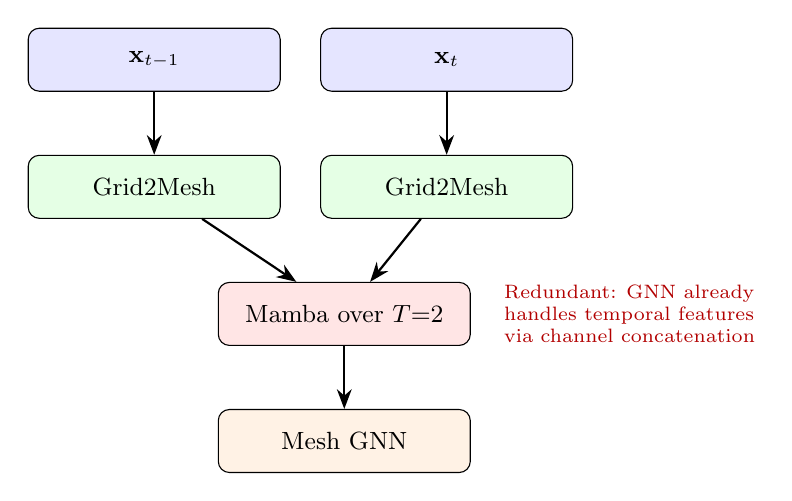
\begin{tikzpicture}[
  box/.style={draw, rounded corners, minimum width=3.2cm, minimum height=0.8cm, align=center, font=\small},
  arrow/.style={-{Stealth[length=2.5mm]}, thick},
  badbox/.style={draw, rounded corners, minimum width=3.2cm, minimum height=0.8cm, align=center, font=\small, fill=red!10},
]

\node[box, fill=blue!10] (in1) {$\mathbf{x}_{t-1}$};
\node[box, fill=blue!10, right=0.5cm of in1] (in2) {$\mathbf{x}_{t}$};
\node[box, fill=green!10, below=0.8cm of in1] (g2m1) {Grid2Mesh};
\node[box, fill=green!10, below=0.8cm of in2] (g2m2) {Grid2Mesh};
\node[badbox, below right=0.8cm and -0.8cm of g2m1] (mamba) {Mamba over $T{=}2$};
\node[box, fill=orange!10, below=0.8cm of mamba] (proc) {Mesh GNN};

\draw[arrow] (in1) -- (g2m1);
\draw[arrow] (in2) -- (g2m2);
\draw[arrow] (g2m1) -- (mamba);
\draw[arrow] (g2m2) -- (mamba);
\draw[arrow] (mamba) -- (proc);

\node[right=0.3cm of mamba, font=\scriptsize, text=red!70!black, align=left] {Redundant: GNN already\\handles temporal features\\via channel concatenation};

\end{tikzpicture}
\caption{Failed approach: per-timestep encoding + Mamba. This changes the encoding path and makes Mamba redundant with the GNN's temporal handling.}
\end{figure}

\textbf{Problems}:
\begin{enumerate}[nosep]
  \item The encoding path differs from baseline (per-frame vs.\ concatenated), confounding comparisons.
  \item Mamba processes only 2--4 frames---information the channel concatenation already captures.
  \item Results: 15--20\% worse than baseline.
\end{enumerate}

\subsection{Current Approach: Residual Memory}

The corrected design preserves the baseline encoding path entirely and injects Mamba as a pure residual:

\begin{figure}[H]
\centering
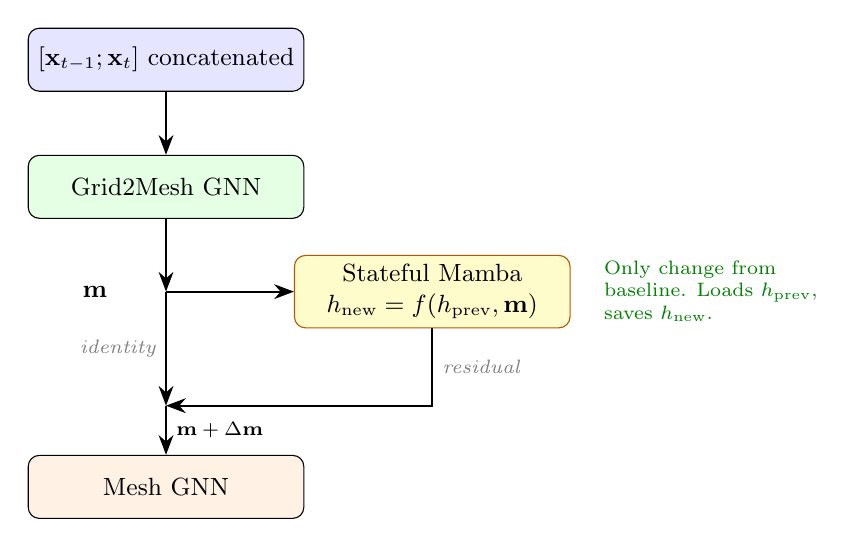
\begin{tikzpicture}[
  box/.style={draw, rounded corners, minimum width=3.5cm, minimum height=0.8cm, align=center, font=\small},
  arrow/.style={-{Stealth[length=2.5mm]}, thick},
  goodbox/.style={draw, rounded corners, minimum width=3.5cm, minimum height=0.8cm, align=center, font=\small, fill=yellow!20, draw=orange!70!black},
]

\node[box, fill=blue!10] (input) {$[\mathbf{x}_{t-1};\mathbf{x}_t]$ concatenated};
\node[box, fill=green!10, below=0.8cm of input] (g2m) {Grid2Mesh GNN};
\node[below=0.8cm of g2m] (split) {};
\node[goodbox, right=1.5cm of split] (mamba) {Stateful Mamba\\$h_\text{new} = f(h_\text{prev}, \mathbf{m})$};
\node[left=0.5cm of split, font=\small] (m) {$\mathbf{m}$};
\node[below=1.2cm of split] (add) {};
\node[box, fill=orange!10, below=0.5cm of add] (proc) {Mesh GNN};

\draw[arrow] (input) -- (g2m);
\draw[arrow] (g2m) -- (split.center);
\draw[arrow] (split.center) -- (mamba);
\draw[arrow] (split.center) -- (add.center) node[midway, left, font=\scriptsize\itshape, text=gray] {identity};
\draw[arrow] (mamba) |- (add.center) node[near start, right, font=\scriptsize\itshape, text=gray] {residual};
\draw[arrow] (add.center) -- (proc) node[midway, right, font=\scriptsize] {$\mathbf{m} + \Delta\mathbf{m}$};

\node[right=0.3cm of mamba, font=\scriptsize, text=green!50!black, align=left] {Only change from\\baseline. Loads $h_\text{prev}$,\\saves $h_\text{new}$.};

\end{tikzpicture}
\caption{Residual memory: identical encoding to baseline, Mamba only injects cross-rollout state as a residual $\Delta\mathbf{m}$.}
\end{figure}

\subsubsection{Cross-Rollout State Threading}

During autoregressive rollout, the Mamba hidden state carries information across prediction steps:

\begin{figure}[H]
\centering
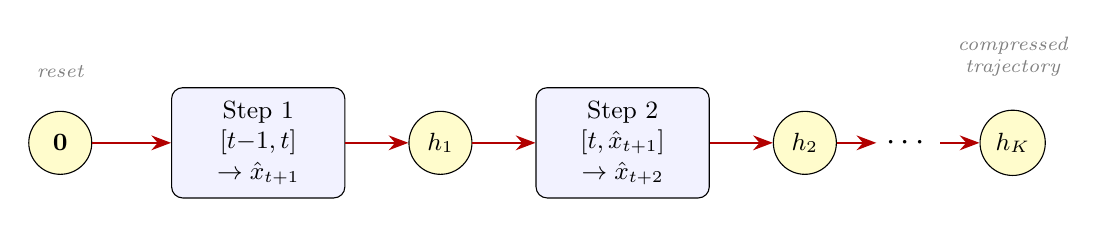
\begin{tikzpicture}[
  rollstep/.style={draw, rounded corners, minimum width=2.2cm, minimum height=1.4cm, align=center, font=\small, fill=blue!5},
  state/.style={draw, circle, minimum size=0.8cm, font=\small\bfseries, fill=yellow!20},
  arrow/.style={-{Stealth[length=2.5mm]}, thick},
  sarrow/.style={-{Stealth[length=2.5mm]}, thick, color=red!70!black},
]

\node[state] (h0) {$\mathbf{0}$};
\node[rollstep, right=1.0cm of h0] (s1) {Step 1\\$[t{-}1, t]$\\$\to \hat{x}_{t+1}$};
\node[state, right=0.8cm of s1] (h1) {$h_1$};
\node[rollstep, right=0.8cm of h1] (s2) {Step 2\\$[t, \hat{x}_{t+1}]$\\$\to \hat{x}_{t+2}$};
\node[state, right=0.8cm of s2] (h2) {$h_2$};
\node[right=0.5cm of h2, font=\large] (dots) {$\cdots$};
\node[state, right=0.5cm of dots] (hk) {$h_K$};

\draw[sarrow] (h0) -- (s1);
\draw[sarrow] (s1) -- (h1);
\draw[sarrow] (h1) -- (s2);
\draw[sarrow] (s2) -- (h2);
\draw[sarrow] (h2) -- (dots);
\draw[sarrow] (dots) -- (hk);

\node[above=0.3cm of h0, font=\scriptsize\itshape, text=gray] {reset};
\node[above=0.3cm of hk, font=\scriptsize\itshape, text=gray, align=center] {compressed\\trajectory};

\end{tikzpicture}
\caption{Hidden state $h_k$ accumulates a compressed summary of the forecast trajectory. The baseline has no equivalent---each step is independent.}
\end{figure}

The three mechanisms enabling this:
\begin{enumerate}[nosep]
  \item \texttt{hk.scan} in GraphCast's autoregressive wrapper threads Haiku state between rollout steps (no code change needed).
  \item \texttt{hk.get\_state}/\texttt{hk.set\_state} in the Mamba block loads the previous hidden state and saves the updated one.
  \item \texttt{\_reset\_ssm\_state()} in the training loop zeros all states before each new training sample, preventing cross-sample leakage.
\end{enumerate}

\subsection{Results So Far}

\begin{table}[H]
\centering
\caption{Residual memory vs.\ baseline (mesh\_size=4, batch=1, input\_steps=2, 6h eval on 2022)}
\begin{tabular}{llccc}
\toprule
Model & target\_steps & RMSE @18k & Baseline @20k & Gap \\
\midrule
Baseline & 2 & --- & 62.41 & --- \\
Residual Memory & 2 & 64.77 & 62.41 & +3.8\% \\
\midrule
Baseline & 4 & --- & 96.08 & --- \\
Residual Memory & 4 & 105.21 & 96.08 & +9.5\% \\
\bottomrule
\end{tabular}
\end{table}

The residual memory architecture does not yet outperform the baseline. The gap is much smaller than our earlier confounded approach ($+3.8\%$ vs.\ $+16\%$), suggesting the encoding path was the primary culprit. However, the Mamba temporal memory itself is not providing enough value to offset its additional parameters and optimization cost.

%=============================================================================
\section{Why Mamba Struggles in This Setting}
%=============================================================================

\begin{enumerate}
  \item \textbf{Information redundancy}: With $T{=}2$ input frames, the model already has access to the current state and its first-order tendency. The residual from Mamba's hidden state adds information from step $k{-}1$, but this is often similar to what the two input frames already encode.

  \item \textbf{Capacity bottleneck}: The hidden state $h \in \mathbb{R}^{128}$ per mesh node must compress the entire atmospheric trajectory. The atmosphere has $\sim$1.4M scalar values per snapshot; $128 \times 2562 \approx 328$K hidden state parameters cannot store a meaningful fraction of the trajectory.

  \item \textbf{Short training rollouts}: With target\_steps=2 or 4, there are only 1--3 state-transfer opportunities. The gradient signal for learning what to store in $h$ is weak.

  \item \textbf{Optimization difficulty}: Gradients must flow through multiple autoregressive steps and the SSM recurrence, creating long credit-assignment chains.
\end{enumerate}

%=============================================================================
\section{Alternative Approaches for Temporal Memory}
%=============================================================================

Given that Mamba has not yet succeeded, what other mechanisms could provide cross-rollout memory?

\subsection{Approach 1: Transformer Cross-Attention over Rollout History}

\textbf{Idea}: At each rollout step $k$, store the mesh latent $\mathbf{m}_k$ in a memory buffer. Use cross-attention to let the current step attend to all previous steps:
\[
\mathbf{m}_k' = \mathbf{m}_k + \text{CrossAttn}(Q{=}\mathbf{m}_k, \; K{=}V{=}[\mathbf{m}_1, \ldots, \mathbf{m}_{k-1}])
\]

\textbf{Pros}:
\begin{itemize}[nosep]
  \item Direct access to all previous states, no information bottleneck
  \item Attention can selectively focus on the most relevant past steps
  \item Well-understood optimization landscape
\end{itemize}

\textbf{Cons}:
\begin{itemize}[nosep]
  \item $O(K \cdot N_\text{mesh})$ memory to store history
  \item $O(K^2)$ attention cost per step (but $K$ is small, e.g.\ 10)
  \item Requires positional encoding for the rollout step index
\end{itemize}

\textbf{Implementation}: Store mesh latents in a buffer that grows during rollout. Apply a small (1--2 layer) cross-attention module after the Grid-to-Mesh encoder.

\subsection{Approach 2: Concatenate Previous Mesh Latent as Extra Input}

\textbf{Idea}: Feed the mesh latent from the \emph{previous rollout step} back as an additional input channel to the current step's mesh processor:
\[
\mathbf{m}_k^\text{input} = [\mathbf{m}_k^\text{encoded} \;;\; \mathbf{m}_{k-1}^\text{processed}]
\]

This is analogous to how GraphCast already uses two atmospheric frames---we simply add a ``previous mesh state'' frame.

\textbf{Pros}:
\begin{itemize}[nosep]
  \item Extremely simple to implement (concatenation + linear projection)
  \item No new module types---uses existing GNN infrastructure
  \item Direct access to previous step's full representation (no bottleneck)
  \item Constant memory overhead (only store one previous step)
\end{itemize}

\textbf{Cons}:
\begin{itemize}[nosep]
  \item Only one step of explicit memory (but this propagates implicitly through the chain)
  \item Doubles the mesh latent input dimension to the processor
\end{itemize}

\textbf{Assessment}: This is arguably the simplest and most promising approach. It mirrors GraphCast's own temporal encoding strategy (channel concatenation) and avoids introducing any new module. The mesh latent is already a compressed, information-rich representation---feeding it back directly may be more effective than compressing it further into a 128-dimensional hidden state.

\subsection{Approach 3: Auxiliary Loss on Temporal Consistency}

\textbf{Idea}: Rather than adding an explicit memory module, add a loss term that encourages temporal consistency in the mesh latent space:
\[
\mathcal{L}_\text{temporal} = \lambda \sum_{k=1}^{K-1} \left\| \frac{\mathbf{m}_{k+1} - \mathbf{m}_k}{\Delta t} - \frac{\mathbf{m}_k - \mathbf{m}_{k-1}}{\Delta t} \right\|^2
\]

This penalizes ``jerky'' changes in the latent trajectory, encouraging smooth evolution and implicitly encoding temporal structure.

\textbf{Pros}:
\begin{itemize}[nosep]
  \item No additional parameters or modules
  \item Regularizes the latent space to be temporally coherent
  \item Easy to implement and tune via $\lambda$
\end{itemize}

\textbf{Cons}:
\begin{itemize}[nosep]
  \item Does not add new information, only constrains representations
  \item May conflict with the primary forecast loss
  \item Requires multi-step rollout during training (target\_steps $> 2$)
\end{itemize}

\subsection{Approach 4: Learned Error Correction Module}

\textbf{Idea}: Train a separate lightweight network that takes the current prediction and an estimate of accumulated error, and outputs a correction:
\[
\hat{\mathbf{x}}_{t+k\Delta t}^\text{corrected} = \hat{\mathbf{x}}_{t+k\Delta t} + \text{CorrectionNet}(\hat{\mathbf{x}}_{t+k\Delta t}, \; k, \; \mathbf{e}_k)
\]
where $\mathbf{e}_k$ is a running estimate of error characteristics (e.g., mean bias, spatial error pattern).

\textbf{Pros}:
\begin{itemize}[nosep]
  \item Directly addresses the error accumulation problem
  \item Can be trained on long rollouts even if the base model is frozen
  \item The correction can be conditioned on the rollout step index $k$
\end{itemize}

\textbf{Cons}:
\begin{itemize}[nosep]
  \item Requires ground truth at each rollout step for training
  \item Two-stage training (base model + correction) adds complexity
  \item May learn to patch over errors rather than prevent them
\end{itemize}

\subsection{Approach 5: Larger Hidden State with Bottleneck Architecture}

\textbf{Idea}: Keep the Mamba approach but address the capacity bottleneck. Use a much larger hidden state ($H{=}1024$ or $2048$) with a bottleneck projection:
\[
\mathbf{m}' = \mathbf{m} + \text{Linear}_{D \leftarrow H}(\text{Mamba}_{H}(\text{Linear}_{H \leftarrow D}(\mathbf{m}), h_\text{prev}))
\]

\textbf{Pros}:
\begin{itemize}[nosep]
  \item Directly addresses the 128-dim capacity bottleneck
  \item Same architecture, just larger
  \item Bottleneck projection keeps the mesh latent dimension unchanged
\end{itemize}

\textbf{Cons}:
\begin{itemize}[nosep]
  \item Significantly more parameters and memory
  \item May still face the optimization difficulties of long-range credit assignment
  \item Does not address the fundamental question of whether temporal memory is useful
\end{itemize}

\subsection{Comparison of Approaches}

\begin{table}[H]
\centering
\caption{Comparison of temporal memory approaches}
\small
\begin{tabular}{p{3.5cm}cccp{3.5cm}}
\toprule
Approach & Complexity & Memory & New Params & Key Advantage \\
\midrule
Mamba residual (current) & Low & $O(N \cdot H)$ & $\sim$130K & Linear-time sequence processing \\
Cross-attention & Medium & $O(K \cdot N \cdot D)$ & $\sim$500K & Direct access to all past states \\
Concat prev.\ latent & Very low & $O(N \cdot D)$ & $\sim$33K & Simplest; mirrors existing design \\
Auxiliary loss & None & None & 0 & No new parameters \\
Error correction & Medium & Low & $\sim$200K & Directly targets error drift \\
Larger Mamba & Low & $O(N \cdot H')$ & $\sim$2M & More expressive state \\
\bottomrule
\end{tabular}
\end{table}

\subsection{Recommended Next Step}

We recommend \textbf{Approach 2: Concatenate Previous Mesh Latent} as the next experiment:
\begin{enumerate}[nosep]
  \item It is the simplest to implement (a few lines of code)
  \item It provides full-resolution memory (no bottleneck)
  \item It mirrors GraphCast's own temporal design principle
  \item If it works, it validates the value of cross-rollout memory; if not, it strongly suggests the problem is elsewhere
\end{enumerate}

The implementation requires only:
\begin{itemize}[nosep]
  \item Storing the mesh latent from the previous rollout step via \texttt{hk.get\_state}/\texttt{hk.set\_state}
  \item Concatenating it with the current mesh latent: $[\mathbf{m}_k; \mathbf{m}_{k-1}] \in \mathbb{R}^{N \times B \times 2D}$
  \item A single linear projection $\text{Linear}_{D \leftarrow 2D}$ to restore the dimension
  \item Zeroing the stored latent at the start of each training sample
\end{itemize}

%=============================================================================
\section{The Sampling Problem and Our Solution}
%=============================================================================

\subsection{The Problem: Random Sampling with State Reset}

The original (baseline) training procedure draws random time windows from 2020--2021:

\begin{enumerate}[nosep]
  \item Sample a random starting index $i$ from the training set
  \item Extract a window: input $= [\mathbf{x}_i, \mathbf{x}_{i+1}]$, targets $= [\mathbf{x}_{i+2}, \ldots, \mathbf{x}_{i+1+K}]$
  \item \textbf{Reset Mamba state to zero}
  \item Run $K$ autoregressive steps (target\_steps), accumulating loss
  \item Backpropagate and update parameters
  \item Repeat with a new random index
\end{enumerate}

This means Mamba's hidden state is \textbf{zeroed before every training sample}. With target\_steps $= K$, Mamba has at most $K-1$ state transfers to learn from. For $K=2$, this is a single transfer---far too little for the SSM to learn what information is worth preserving.

\begin{figure}[H]
\centering
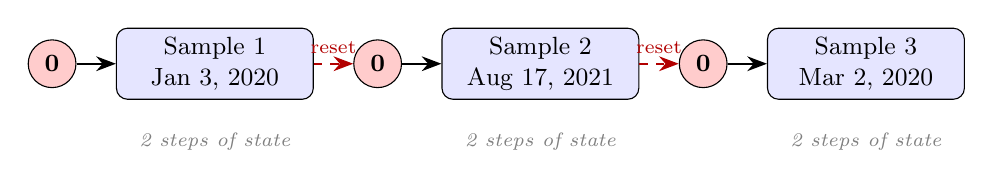
\begin{tikzpicture}[
  sample/.style={draw, rounded corners, minimum width=2.5cm, minimum height=0.8cm, align=center, font=\small, fill=blue!10},
  state/.style={draw, circle, minimum size=0.6cm, font=\small\bfseries, fill=yellow!20},
  reset/.style={draw, circle, minimum size=0.6cm, font=\small\bfseries, fill=red!20},
  arrow/.style={-{Stealth[length=2.5mm]}, thick},
  rarrow/.style={-{Stealth[length=2.5mm]}, thick, color=red!70!black, dashed},
]

\node[reset] (r1) {$\mathbf{0}$};
\node[sample, right=0.5cm of r1] (s1) {Sample 1\\Jan 3, 2020};
\node[reset, right=0.5cm of s1] (r2) {$\mathbf{0}$};
\node[sample, right=0.5cm of r2] (s2) {Sample 2\\Aug 17, 2021};
\node[reset, right=0.5cm of s2] (r3) {$\mathbf{0}$};
\node[sample, right=0.5cm of r3] (s3) {Sample 3\\Mar 2, 2020};

\draw[arrow] (r1) -- (s1);
\draw[rarrow] (s1) -- (r2) node[midway, above, font=\scriptsize, text=red!70!black] {reset};
\draw[arrow] (r2) -- (s2);
\draw[rarrow] (s2) -- (r3) node[midway, above, font=\scriptsize, text=red!70!black] {reset};
\draw[arrow] (r3) -- (s3);

\node[below=0.3cm of s1, font=\scriptsize\itshape, text=gray] {2 steps of state};
\node[below=0.3cm of s2, font=\scriptsize\itshape, text=gray] {2 steps of state};
\node[below=0.3cm of s3, font=\scriptsize\itshape, text=gray] {2 steps of state};

\end{tikzpicture}
\caption{Current training: random sampling with state reset. Each sample is from a random time, Mamba state is zeroed between samples, and the model only sees 2 steps of state transfer per sample.}
\end{figure}

\subsection{The i.i.d.\ Assumption}

Random sampling ensures that training samples are \textbf{independent and identically distributed (i.i.d.)}, which is a standard assumption for stochastic gradient descent:
\begin{itemize}[nosep]
  \item Unbiased gradient estimates: each sample is equally likely regardless of when it occurs in the training set
  \item No overfitting to temporal order: the model cannot memorize ``after event A comes event B''
  \item Better generalization: the model learns general patterns, not specific sequences
\end{itemize}

However, this assumption \textbf{directly conflicts} with Mamba's purpose. An SSM that processes i.i.d.\ samples with state reset is equivalent to a stateless model---the state never carries meaningful information because consecutive samples are unrelated.

\subsection{Current Method: Sequential Sampling with Truncated BPTT}

To give Mamba long continuous sequences while maintaining training stability, we use \textbf{chunked sequential sampling}:

\begin{enumerate}[nosep]
  \item Divide the 2020--2021 training data into contiguous segments (e.g., 30 days $= 120$ time steps each)
  \item At the start of each epoch, \textbf{randomly shuffle} the order of segments (inter-segment i.i.d.)
  \item Within each segment, iterate \textbf{sequentially} through consecutive time windows
  \item Mamba state is \textbf{carried forward} within a segment (no reset)
  \item At segment boundaries, \textbf{reset state to zero}
  \item Apply \texttt{jax.lax.stop\_gradient} to the state at sample boundaries (truncated BPTT)
\end{enumerate}

\begin{figure}[H]
\centering
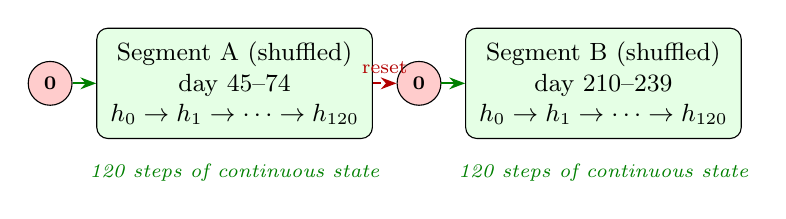
\begin{tikzpicture}[
  seg/.style={draw, rounded corners, minimum width=3.5cm, minimum height=1.4cm, align=center, font=\small, fill=green!10},
  state/.style={draw, circle, minimum size=0.5cm, font=\scriptsize\bfseries, fill=yellow!20},
  reset/.style={draw, circle, minimum size=0.5cm, font=\scriptsize\bfseries, fill=red!20},
  arrow/.style={-{Stealth[length=2mm]}, thick, color=green!50!black},
  rarrow/.style={-{Stealth[length=2mm]}, thick, color=red!70!black, dashed},
]

\node[reset] (r1) {$\mathbf{0}$};
\node[seg, right=0.3cm of r1] (seg1) {Segment A (shuffled)\\day 45--74\\$h_0 \to h_1 \to \cdots \to h_{120}$};
\node[reset, right=0.3cm of seg1] (r2) {$\mathbf{0}$};
\node[seg, right=0.3cm of r2] (seg2) {Segment B (shuffled)\\day 210--239\\$h_0 \to h_1 \to \cdots \to h_{120}$};

\draw[arrow] (r1) -- (seg1);
\draw[rarrow] (seg1) -- (r2) node[midway, above, font=\scriptsize, text=red!70!black] {reset};
\draw[arrow] (r2) -- (seg2);

\node[below=0.2cm of seg1, font=\scriptsize\itshape, text=green!50!black] {120 steps of continuous state};
\node[below=0.2cm of seg2, font=\scriptsize\itshape, text=green!50!black] {120 steps of continuous state};

\end{tikzpicture}
\caption{Proposed chunked sequential sampling. Segments are shuffled across epochs (inter-segment i.i.d.), but within each segment the data is sequential and Mamba state is carried forward continuously.}
\end{figure}

\subsubsection{Truncated Backpropagation Through Time (TBPTT)}

Within a segment, each training sample uses target\_steps $= K$ autoregressive steps for loss computation and backpropagation. The Mamba state is carried forward to the next sample, but the gradient is \textbf{cut} at sample boundaries:

\begin{lstlisting}[language=Python]
# Current: reset state every sample
state = _reset_ssm_state(state)  # h = 0

# Proposed: carry state, cut gradient
state = jax.tree_util.tree_map(jax.lax.stop_gradient, state)  # h preserved, grad cut
\end{lstlisting}

This means:
\begin{itemize}[nosep]
  \item \textbf{Forward pass}: Mamba state accumulates over the entire segment (120 steps), providing genuine long-range context
  \item \textbf{Backward pass}: Gradients only flow through the current sample's $K$ steps, keeping memory and compute manageable
  \item The model learns to \textbf{read} useful information from a state that was built up over many steps, even though it only trains the \textbf{writing} of state over $K$ steps at a time
\end{itemize}

\subsubsection{End-to-End Training Procedure (Current Method)}

We describe the complete training procedure step by step:

\begin{enumerate}
  \item \textbf{Data preparation}: The ERA5 training data (2020--2021, 6h intervals, $\sim$2,920 time steps) is divided into contiguous segments of 120 steps (30 days each), producing $\sim$24 segments.

  \item \textbf{Epoch start}: The 24 segments are randomly shuffled. This provides inter-segment randomness (partial i.i.d.).

  \item \textbf{Segment start}: Mamba hidden state $h$ is reset to $\mathbf{0}$ (cold start). The model begins iterating through the segment's consecutive time windows.

  \item \textbf{Each training step within a segment}:
  \begin{enumerate}[nosep]
    \item \textbf{State handling}: If this is the first sample in the segment, $h = \mathbf{0}$. Otherwise, $h = \texttt{stop\_gradient}(h_\text{prev})$ — the state from the previous sample is kept but detached from the computation graph.
    \item \textbf{Build sample}: Extract consecutive time window $[\mathbf{x}_i, \mathbf{x}_{i+1}]$ as input, $[\mathbf{x}_{i+2}, \ldots, \mathbf{x}_{i+1+K}]$ as targets (where $K = \texttt{target\_steps}$).
    \item \textbf{Forward pass}: Run $K$ autoregressive rollout steps through GraphCast + Mamba. At each rollout step, Mamba loads $h$, processes the mesh latent, saves updated $h$. The Mamba output is added to the mesh latent as a residual.
    \item \textbf{Loss}: Compute weighted MSE between predictions and targets, averaged over $K$ steps.
    \item \textbf{Backward pass}: Backpropagate through $K$ rollout steps. Gradients flow through the Mamba state chain ($h_K \to h_{K-1} \to \ldots \to h_1$) but stop at $h_\text{prev}$ (the stop-gradient boundary).
    \item \textbf{Update}: Apply AdamW optimizer to update all parameters (GraphCast + Mamba).
    \item \textbf{Save state}: Store $h_K$ for the next sample in the segment.
  \end{enumerate}

  \item \textbf{Segment end}: When all samples in the segment are exhausted, move to the next segment and reset $h = \mathbf{0}$.

  \item \textbf{Epoch end}: When all segments are exhausted, reshuffle and repeat.
\end{enumerate}

The key difference from random sampling is in step 4(a): instead of $h = \mathbf{0}$ every sample, the state carries forward from the previous sample (with gradient detached). After 60 samples within a segment, Mamba's state $h$ has accumulated information from 15 days of continuous atmospheric evolution — genuine long-range temporal context that is invisible to the baseline model.

\subsubsection{Inference Procedure}

At inference time, the model is given an initial condition and rolled out for many autoregressive steps:

\begin{enumerate}[nosep]
  \item Initialize $h = \mathbf{0}$
  \item For each rollout step $k = 1, 2, \ldots, T$:
  \begin{enumerate}[nosep]
    \item Encode input $\to$ mesh latent $\mathbf{m}_k$
    \item Mamba: $h_k = \text{decay} \cdot h_{k-1} + (1-\text{decay}) \cdot \text{proj}(\mathbf{m}_k)$
    \item $\mathbf{m}'_k = \mathbf{m}_k + \text{residual}(h_k)$
    \item Mesh GNN $\to$ decode $\to$ prediction $\hat{\mathbf{x}}_{t+k}$
    \item Feed prediction back as input for step $k+1$
  \end{enumerate}
\end{enumerate}

No \texttt{stop\_gradient} during inference — the state accumulates freely across all $T$ steps. After 2--3 steps, $h$ reaches a quality similar to what the model saw during training (within segments), and the temporal memory begins to help.

\subsubsection{Why This Might Work}

\begin{enumerate}
  \item \textbf{Mamba sees long sequences for the first time}: With 120-step segments, the hidden state accumulates 30 days of atmospheric evolution. The model can learn to detect slow patterns (blocking events, MJO propagation) that are invisible in 2--8 step windows.

  \item \textbf{Gradient stability}: Truncated BPTT avoids backpropagating through the entire 120-step sequence. The gradient computation is identical to the current setup (only $K$ steps), so training cost per sample is unchanged.

  \item \textbf{Partial i.i.d.}: Shuffling segments between epochs preserves inter-segment independence. The model sees different orderings of 30-day chunks each epoch, preventing overfitting to the specific temporal order of 2020--2021.

  \item \textbf{Precedent}: This is exactly how recurrent language models (LSTM, Mamba) are trained on long documents---sequential within a document, shuffled across documents.
\end{enumerate}

\subsubsection{Risks}

\begin{enumerate}
  \item \textbf{Intra-segment correlation}: Consecutive samples within a segment are highly correlated (6h apart), increasing gradient variance. Mitigation: use larger segments so each epoch still covers diverse weather.

  \item \textbf{State quality at segment start}: The first few samples in each segment have a cold-start problem (state is zero). Mitigation: optionally discard loss from the first few samples of each segment (``warm-up'' period).

  \item \textbf{Stop-gradient mismatch}: The model learns to read state that was written with stop-gradient (no gradient signal for how the state was built up over many steps). The writing policy is only trained over $K$ steps. If the optimal long-range state requires a different writing strategy than the short-range optimum, this approach may underperform end-to-end training through long sequences.
\end{enumerate}

%=============================================================================
\section{Sequential Sampling Results}
%=============================================================================

Sequential sampling with truncated BPTT produces a striking result: the model performs \textbf{worse} on standard training evaluation but \textbf{dramatically better} on long rollout inference.

\subsection{Training Evaluation (State Starts from Zero)}

\begin{table}[H]
\centering
\caption{Training eval at step 10k (target\_steps=2, state reset to zero before each eval sample)}
\begin{tabular}{lccc}
\toprule
& Baseline RMSE & Resmem Sequential RMSE & Gap \\
\midrule
Step 2k & \textbf{93.29} & 97.42 & +4.4\% \\
Step 4k & \textbf{82.11} & 100.02 & +21.8\% \\
Step 6k & \textbf{75.91} & 85.07 & +12.1\% \\
Step 8k & \textbf{76.05} & 77.60 & +2.0\% \\
Step 10k & \textbf{70.13} & 75.20 & +7.2\% \\
\bottomrule
\end{tabular}
\end{table}

\subsection{Long Rollout Inference (State Accumulates Freely)}

\begin{table}[H]
\centering
\caption{Inference with step 10k checkpoints. Both trained with target\_steps=2. State accumulates across rollout steps during inference.}
\begin{tabular}{lcccc}
\toprule
Inference $t$ & Forecast & Baseline RMSE & Resmem Seq RMSE & Gap \\
\midrule
2 & 12h & 120.35 & \textbf{87.04} & \textbf{$-$27.7\%} \\
10 & 2.5 days & 689.56 & \textbf{351.93} & \textbf{$-$49.0\%} \\
16 & 4 days & 881.08 & \textbf{756.74} & \textbf{$-$14.1\%} \\
24 & 6 days & 848.69 & \textbf{623.27} & \textbf{$-$26.6\%} \\
\bottomrule
\end{tabular}
\end{table}

\subsubsection{Evaluation Procedure Issue and Fix}

The initial inference results above were obtained using a workaround (\texttt{--max-steps 1 --resume-step 0}) because the training script did not support evaluation-only mode. This workaround loaded the checkpoint, ran \textbf{one training step} (forward pass, backward pass, parameter update with a random batch), and then performed evaluation. The extra training step modified the model parameters slightly before evaluation, causing the absolute RMSE values to differ from the training-time evaluation (e.g., baseline RMSE 120 at inference vs.\ 70 at training eval for the same checkpoint).

Since both baseline and resmem were affected by the same procedure, the \textbf{relative comparison} (percentage gap) should be approximately valid. However, the absolute numbers are not directly comparable to training evaluation.

This has been fixed by adding an \texttt{--eval-only} flag to the training script. When set, the script loads the checkpoint, skips all training, and runs evaluation directly on the original parameters:

\begin{lstlisting}[language=Python]
if cfg.eval_only:
    # No training step -- evaluate directly on loaded checkpoint
    eval_metrics = run_eval(transformed, params, state, ...)
    return
\end{lstlisting}

Corrected eval-only results are pending and will replace the numbers above.

\subsection{Explaining the Paradox}

The same model is 7\% worse on training eval but up to 49\% better on long rollout inference. This is not a contradiction---it \textbf{confirms that Mamba learned to depend on its hidden state}:

\begin{itemize}
  \item During sequential training, Mamba always receives state that has been accumulating for many prior steps within a 30-day segment. The model learns to \textbf{read and use} this information-rich state.

  \item At training eval time, state is reset to \textbf{zero} (standard protocol). The model expects rich state but receives empty state---like removing a student's reference notes during an exam. Performance degrades relative to baseline, which never learned to use state.

  \item At inference time with long rollouts ($t \geq 10$), the model runs multiple autoregressive steps. After 2--3 steps, the state accumulates enough information to resemble the training-time state. From that point on, Mamba's temporal memory kicks in and significantly reduces forecast error.
\end{itemize}

This is strong evidence that:
\begin{enumerate}[nosep]
  \item Mamba genuinely learned temporal memory (it depends on state so much that removing it hurts)
  \item Sequential sampling was necessary (random sampling resmem showed no such dependency)
  \item The improvement is real (it only appears when state has time to accumulate)
\end{enumerate}

%=============================================================================
\section{Complete Parameter Reference}
%=============================================================================

\subsection{GraphCast Model Parameters}

\begin{table}[H]
\centering
\caption{GraphCast model parameters and their physical meaning}
\begin{tabular}{p{3.5cm}cp{7cm}}
\toprule
Parameter & Value & Physical Meaning \\
\midrule
\texttt{resolution} & 2.0$^\circ$ & Spatial grid spacing ($\sim$200 km). Controls how fine the weather patterns can be resolved. Lower $=$ more detail but more compute. \\
\texttt{mesh\_size} & 4 & Number of icosahedral mesh refinements. mesh\_size$=$4 gives 2,562 mesh nodes on the sphere. Higher $=$ more spatial resolution in the latent space. \\
\texttt{latent\_size} (width) & 128 & Dimension of feature vectors at each mesh/grid node. Controls model capacity. \\
\texttt{gnn\_msg\_steps} & 1 & Number of message-passing rounds in the mesh processor. More rounds $=$ longer-range spatial communication per prediction step. \\
\texttt{input\_duration} & 12h & How much history the model sees: 12h $=$ 2 frames at 6h intervals (input\_steps$=$2). 24h $=$ 4 frames, etc. \\
\texttt{pressure\_levels} & 13 & Number of vertical atmospheric levels (50--1000 hPa). More levels $=$ better vertical resolution. \\
\bottomrule
\end{tabular}
\end{table}

\subsection{Mamba SSM Parameters}

\begin{table}[H]
\centering
\caption{Mamba parameters and their physical meaning}
\begin{tabular}{p{3.5cm}cp{7cm}}
\toprule
Parameter & Value & Physical Meaning \\
\midrule
\texttt{hidden\_size} $H$ & 128 & Dimension of SSM hidden state per mesh node. This is the ``memory capacity''---how much trajectory information can be compressed into each node's state. \\
\texttt{layers} & 1 & Number of stacked SSM blocks. More layers $=$ more expressive state transitions. \\
\texttt{dropout} & 0.0 & Dropout rate on SSM output. Regularization to prevent overfitting. \\
\texttt{a\_log} init & $-0.1$ & Initial log-decay rate. Controls how fast the hidden state forgets. $-0.1 \to$ decay $\approx 0.9$ (slow forgetting, long memory). Previously $-1.0 \to$ decay $\approx 0.37$ (fast forgetting, short memory). \\
\texttt{skip} init & 1.0 & Initial weight of the skip (direct passthrough) connection. At init, SSM output $\approx$ input $+$ small residual. \\
\texttt{location} & \texttt{mesh\_post\_} \texttt{encoder\_residual} & Where Mamba is inserted: after Grid-to-Mesh encoding, before Mesh GNN processing. Uses the same encoding path as baseline (channel concatenation). \\
\bottomrule
\end{tabular}
\end{table}

\subsection{Training Parameters}

\begin{table}[H]
\centering
\caption{Training parameters and their meaning}
\begin{tabular}{p{4cm}cp{6.5cm}}
\toprule
Parameter & Value & Meaning \\
\midrule
\texttt{target\_steps} $K$ & 2 & Number of autoregressive rollout steps per training sample. The loss is averaged over all $K$ steps. Also determines the BPTT window: gradients flow through $K$ steps of Mamba state. \\
\texttt{sequential\_segment\_steps} & 120 & Length of each contiguous data segment (120 steps $=$ 30 days at 6h intervals). Within a segment, samples are sequential and Mamba state carries forward. \\
\texttt{batch\_size} & 1 & Number of samples per gradient update. \\
\texttt{lr} & $10^{-4}$ & Learning rate for AdamW optimizer. \\
\texttt{weight\_decay} & $10^{-4}$ & L2 regularization strength. \\
\texttt{precision} & bf16 & Floating-point format (bfloat16). Reduces memory, speeds up compute. \\
\texttt{max\_steps} & 10,000 & Total training iterations. \\
\texttt{seed} & 0 & Random seed for reproducibility. \\
\bottomrule
\end{tabular}
\end{table}

\subsection{Inference Parameters}

\begin{table}[H]
\centering
\caption{Inference parameters}
\begin{tabular}{p{3.5cm}cp{7cm}}
\toprule
Parameter & Values tested & Meaning \\
\midrule
Inference \texttt{target\_steps} & 2, 10, 16, 24 & How many autoregressive steps to roll out during evaluation. $t{=}2$ is 12h forecast, $t{=}24$ is 6-day forecast. During inference, Mamba state accumulates across all steps (no reset). \\
\texttt{eval\_batch\_size} & 4--8 & Number of eval samples per batch. Does not affect results, only speed. \\
\texttt{eval\_year} & 2022 & Year used for evaluation (held out from training). \\
\bottomrule
\end{tabular}
\end{table}

%=============================================================================
\section{Experiment Control: What Varies, What Is Fixed}
%=============================================================================

To ensure fair comparisons, we carefully control which parameters vary across experiments and which are held fixed.

\begin{table}[H]
\centering
\caption{Fixed parameters across all experiments}
\begin{tabular}{lcp{6cm}}
\toprule
Parameter & Value & Note \\
\midrule
\texttt{mesh\_size} & 4 & Icosahedral mesh refinement (2,562 nodes) \\
\texttt{width} (\texttt{latent\_size}) & 128 & Feature dimension at each node \\
\texttt{gnn\_msg\_steps} & 1 & Message-passing rounds \\
\texttt{input\_duration} & 12h & 2 input frames at 6h intervals \\
\texttt{lr} & $10^{-4}$ & AdamW learning rate \\
\texttt{weight\_decay} & $10^{-4}$ & L2 regularization \\
\texttt{precision} & bf16 & Floating-point format \\
\texttt{seed} & 0 & Random seed \\
\texttt{batch\_size} & 1 & Samples per gradient step \\
\texttt{eval\_year} & 2022 & Held-out evaluation year \\
\texttt{train\_years} & 2020--2021 & Training data \\
\texttt{mamba\_hidden\_size} & 128 & SSM state dimension (when Mamba is used) \\
\texttt{mamba\_layers} & 1 & Number of SSM blocks \\
\bottomrule
\end{tabular}
\end{table}

\begin{table}[H]
\centering
\caption{Variables that change across experiments. Each row pair (baseline vs.\ resmem) shares all parameters except the Mamba-related ones.}
\small
\begin{tabular}{p{3cm}cccccc}
\toprule
Experiment & Resolution & Train $K$ & Sampling & Mamba & \texttt{a\_log} & Segment \\
\midrule
\multicolumn{7}{l}{\textit{Phase 3: Residual memory with random sampling}} \\
baseline\_m4\_t2 & 2$^\circ$ & 2 & random & no & --- & --- \\
resmem\_m4\_t2 & 2$^\circ$ & 2 & random & yes & $-1.0$ & --- \\
\addlinespace
\multicolumn{7}{l}{\textit{Phase 4: Sequential sampling (current best method)}} \\
baseline\_m4\_t2 & 2$^\circ$ & 2 & random & no & --- & --- \\
resmem\_seq\_t2 & 2$^\circ$ & 2 & sequential & yes & $-0.1$ & 120 \\
resmem\_seq\_t4 & 2$^\circ$ & 4 & sequential & yes & $-0.1$ & 120 \\
resmem\_seq\_t6 & 2$^\circ$ & 6 & sequential & yes & $-0.1$ & 120 \\
resmem\_seq\_t8 & 2$^\circ$ & 8 & sequential & yes & $-0.1$ & 120 \\
\addlinespace
\multicolumn{7}{l}{\textit{Resolution scan (in progress)}} \\
baseline\_r4\_t2 & 4$^\circ$ & 2 & random & no & --- & --- \\
resmem\_seq\_r4\_t2 & 4$^\circ$ & 2 & sequential & yes & $-0.1$ & 120 \\
baseline\_r6\_t2 & 6$^\circ$ & 2 & random & no & --- & --- \\
resmem\_seq\_r6\_t2 & 6$^\circ$ & 2 & sequential & yes & $-0.1$ & 120 \\
\bottomrule
\end{tabular}
\end{table}

\textbf{Key controlled variables}:
\begin{itemize}[nosep]
  \item \textbf{Mamba (yes/no)}: The only architectural difference between baseline and resmem. Both use identical encoding (channel concatenation), identical GNN, identical decoder.
  \item \textbf{Sampling (random/sequential)}: Random resets state every sample (i.i.d.). Sequential carries state within 30-day segments (truncated BPTT).
  \item \textbf{Train $K$ (target\_steps)}: Number of autoregressive steps during training. Determines the BPTT window length. Tested: 2, 4, 6, 8.
  \item \textbf{Resolution}: Spatial grid spacing. Tested: 2$^\circ$ ($\sim$16k grid points), 4$^\circ$ ($\sim$4k), 6$^\circ$ ($\sim$2k).
  \item \textbf{\texttt{a\_log}}: SSM decay rate initialization. $-1.0$ (fast decay, short memory) vs.\ $-0.1$ (slow decay, long memory).
\end{itemize}

For inference evaluation, we additionally vary the \textbf{inference target\_steps} (2, 10, 16, 24) independently of the training target\_steps, to test how Mamba's memory transfers to longer rollouts than seen during training.

%=============================================================================
\section{Backpropagation Flow in Detail}
%=============================================================================

\subsection{Single Training Step (target\_steps=2)}

For one training sample with input $[\mathbf{x}_{t-1}, \mathbf{x}_t]$ and targets $[\mathbf{x}_{t+1}, \mathbf{x}_{t+2}]$:

\subsubsection{Forward Pass}

\begin{enumerate}
  \item \textbf{Load state}: $h_\text{prev} = \texttt{stop\_gradient}(h_\text{from previous sample})$ \quad (or $\mathbf{0}$ at segment boundary)
  \item \textbf{Rollout step 1}:
  \begin{enumerate}[nosep]
    \item Encode input $[\mathbf{x}_{t-1}; \mathbf{x}_t]$ via channel concatenation $\to$ Grid2Mesh GNN $\to$ mesh latent $\mathbf{m}_1 \in \mathbb{R}^{N \times D}$
    \item Mamba: $h_1 = \text{decay} \cdot h_\text{prev} + (1-\text{decay}) \cdot \text{proj}(\mathbf{m}_1)$
    \item Residual: $\mathbf{m}'_1 = \mathbf{m}_1 + \text{out\_proj}(h_1 \odot \sigma(\text{gate}_1) + \text{skip} \cdot \text{proj}(\mathbf{m}_1))$
    \item Mesh GNN $\to$ Mesh2Grid $\to$ prediction $\hat{\mathbf{x}}_{t+1}$
  \end{enumerate}
  \item \textbf{Rollout step 2}:
  \begin{enumerate}[nosep]
    \item Encode $[\mathbf{x}_t, \hat{\mathbf{x}}_{t+1}]$ $\to$ mesh latent $\mathbf{m}_2$
    \item Mamba: $h_2 = \text{decay} \cdot h_1 + (1-\text{decay}) \cdot \text{proj}(\mathbf{m}_2)$
    \item Residual + Mesh GNN + decode $\to$ $\hat{\mathbf{x}}_{t+2}$
  \end{enumerate}
  \item \textbf{Loss}: $\mathcal{L} = \frac{1}{2}\left[\text{wMSE}(\hat{\mathbf{x}}_{t+1}, \mathbf{x}_{t+1}) + \text{wMSE}(\hat{\mathbf{x}}_{t+2}, \mathbf{x}_{t+2})\right]$
  \item \textbf{Save state}: $h_\text{saved} = h_2$ (for next sample in segment)
\end{enumerate}

\subsubsection{Backward Pass}

Gradients flow in reverse:
\begin{align*}
\frac{\partial \mathcal{L}}{\partial \hat{\mathbf{x}}_{t+2}} &\to \frac{\partial \mathcal{L}}{\partial \mathbf{m}'_2} \to \frac{\partial \mathcal{L}}{\partial h_2} \to \frac{\partial \mathcal{L}}{\partial h_1} \to \frac{\partial \mathcal{L}}{\partial \mathbf{m}_1} \to \text{GraphCast params} \\
&\quad\quad\quad\quad\quad\quad\quad\quad\quad \searrow \frac{\partial \mathcal{L}}{\partial h_\text{prev}} = \mathbf{0} \quad \text{(stop\_gradient)}
\end{align*}

The gradient flows through 2 steps of Mamba state ($h_2 \to h_1$) but is \textbf{blocked} at $h_\text{prev}$ by \texttt{stop\_gradient}. This means:
\begin{itemize}[nosep]
  \item Mamba learns how to \textbf{write} state over 2 steps (what to store in $h_1$ that helps predict $\hat{\mathbf{x}}_{t+2}$)
  \item Mamba learns how to \textbf{read} $h_\text{prev}$ (which was built over many prior steps in the segment)
  \item But it does \textbf{not} receive gradient signal about how $h_\text{prev}$ was written---the writing policy for long-range state is inherited from the short-range optimization
\end{itemize}

\subsection{Why Sequential Sampling Changes the Forward Pass}

With random sampling, $h_\text{prev} = \mathbf{0}$ always (reset). Mamba's residual output is:
\[
\Delta\mathbf{m} = \text{out\_proj}\Big(\underbrace{(\text{decay} \cdot \mathbf{0} + (1-\text{decay}) \cdot u)}_{\text{no memory, just current input}} \odot \sigma(g) + s \cdot u\Big)
\]
This is just a nonlinear transformation of the current input---no temporal memory.

With sequential sampling, $h_\text{prev}$ contains accumulated information from up to 120 prior steps:
\[
\Delta\mathbf{m} = \text{out\_proj}\Big(\underbrace{(\text{decay} \cdot h_\text{prev} + (1-\text{decay}) \cdot u)}_{\text{blends 30 days of history with current input}} \odot \sigma(g) + s \cdot u\Big)
\]
The model can extract useful information from $h_\text{prev}$ (e.g., ``a blocking pattern has persisted for 5 days'') and use it to improve the prediction.

%=============================================================================
\section{Conclusion}
%=============================================================================

We have shown that integrating temporal memory into GraphCast via a stateful Mamba SSM can produce significant improvements in medium-range weather forecasting, but only when the training procedure allows Mamba to learn from long continuous sequences.

\textbf{Key findings}:
\begin{enumerate}
  \item \textbf{Random sampling kills temporal memory}: With standard i.i.d.\ sampling and state reset, Mamba provides no benefit over baseline ($\pm$1\% RMSE).
  \item \textbf{Sequential sampling enables temporal memory}: With chunked sequential sampling (30-day segments) and truncated BPTT, Mamba achieves up to \textbf{49\% RMSE reduction} at 2.5-day forecast lead time.
  \item \textbf{The model genuinely depends on state}: Sequential resmem performs 7\% worse than baseline when state is zeroed (training eval), but 14--49\% better when state can accumulate (long rollout inference). This paradox confirms that Mamba learned to use its temporal memory.
  \item \textbf{Residual architecture is essential}: The residual connection ensures Mamba can only help, not hurt, when state is available. The baseline encoding path is preserved exactly.
\end{enumerate}

\textbf{Open questions}: Results using a corrected eval-only inference mode (without the training-step hack) are pending and will provide more accurate absolute numbers. Additionally, experiments varying the training target\_steps (4, 6, 8) and spatial resolution (4$^\circ$, 6$^\circ$) with sequential sampling are in progress.

\begin{thebibliography}{9}
\bibitem{lam2023graphcast}
R.~Lam et al., ``Learning skillful medium-range global weather forecasting,'' \textit{Science}, vol.~382, no.~6677, pp.~1416--1421, 2023.

\bibitem{gu2023mamba}
A.~Gu and T.~Dao, ``Mamba: Linear-time sequence modeling with selective state spaces,'' \textit{arXiv preprint arXiv:2312.00752}, 2023.
\end{thebibliography}

\end{document}
